% Prepare the two results figures before Figure 7, preserving reference numbers.
\newsavebox{\resultspanels}
\begin{lrbox}{\resultspanels}
\begin{minipage}{\textwidth}
\captionsetup{hypcap=false}
\centering
\begin{minipage}[c]{0.49\textwidth}
\footnotesize
\setlength{\tabcolsep}{2pt}
\renewcommand{\arraystretch}{1.0}
\centering
\captionsetup{font=footnotesize}
\captionof{table}{Comparison of \textbf{Unified EB} vs.\ \textbf{RES} across benchmarks ($\text{EB}=0.1, \text{max\_dns}=48$). Scores report \textbf{Avg@20} $\pm$ 95\% CI (Pass@1 averaged across 20 seeds; 5 seeds for LiveCodeBench). Relative TPF deltas are shown underneath.}
\label{tab:eb_unified_vs_rolling}
\vspace{4pt}
\begin{tabular*}{\linewidth}{@{\extracolsep{\fill}}lcccc@{}}
\toprule
& \multicolumn{2}{c}{\textbf{Unified EB}} & \multicolumn{2}{c}{\textbf{RES}} \\
\cmidrule(lr){2-3} \cmidrule(lr){4-5}
\textbf{Task} & \textbf{Avg@20} & \textbf{TPF} & \textbf{Avg@20} & \textbf{TPF} \\
\midrule
LiveCodeBench & \begin{tabular}[t]{@{}c@{}}65.4\% \\ \scriptsize{($\pm$3.2\%)}\end{tabular} & 18.7 & \begin{tabular}[t]{@{}c@{}}62.6\% \\ \scriptsize{($\pm$3.2\%)}\end{tabular} & \begin{tabular}[t]{@{}c@{}}\textbf{26.3} \\ \scriptsize{(+40.6\%)}\end{tabular} \\
\addlinespace[2pt]
Natural2Code & \begin{tabular}[t]{@{}c@{}}\textbf{93.0\%} \\ \scriptsize{\textbf{($\pm$0.8\%)}}\end{tabular} & 22.9 & \begin{tabular}[t]{@{}c@{}}91.3\% \\ \scriptsize{($\pm$0.9\%)}\end{tabular} & \begin{tabular}[t]{@{}c@{}}\textbf{30.1} \\ \scriptsize{(+31.7\%)}\end{tabular} \\
\addlinespace[2pt]
GPQA Diamond & \begin{tabular}[t]{@{}c@{}}67.5\% \\ \scriptsize{($\pm$1.5\%)}\end{tabular} & 16.6 & \begin{tabular}[t]{@{}c@{}}68.3\% \\ \scriptsize{($\pm$1.4\%)}\end{tabular} & \begin{tabular}[t]{@{}c@{}}\textbf{23.8} \\ \scriptsize{(+43.1\%)}\end{tabular} \\
\addlinespace[2pt]
HiddenMath   & \begin{tabular}[t]{@{}c@{}}\textbf{73.9\%} \\ \scriptsize{\textbf{($\pm$0.9\%)}}\end{tabular} & 22.1 & \begin{tabular}[t]{@{}c@{}}72.6\% \\ \scriptsize{($\pm$0.9\%)}\end{tabular} & \begin{tabular}[t]{@{}c@{}}\textbf{27.2} \\ \scriptsize{(+23.2\%)}\end{tabular} \\
\addlinespace[2pt]
GSM8k        & \begin{tabular}[t]{@{}c@{}}\textbf{92.1\%} \\ \scriptsize{\textbf{($\pm$0.3\%)}}\end{tabular} & 21.7 & \begin{tabular}[t]{@{}c@{}}91.6\% \\ \scriptsize{($\pm$0.3\%)}\end{tabular} & \begin{tabular}[t]{@{}c@{}}\textbf{27.7} \\ \scriptsize{(+28.0\%)}\end{tabular} \\
\addlinespace[2pt]
IFEval       & \begin{tabular}[t]{@{}c@{}}\textbf{93.1\%} \\ \scriptsize{\textbf{($\pm$0.5\%)}}\end{tabular} & 16.8 & \begin{tabular}[t]{@{}c@{}}82.4\% \\ \scriptsize{($\pm$0.7\%)}\end{tabular} & \begin{tabular}[t]{@{}c@{}}\textbf{22.6} \\ \scriptsize{(+34.4\%)}\end{tabular} \\
\addlinespace[2pt]
MMLU         & \begin{tabular}[t]{@{}c@{}}80.3\% \\ \scriptsize{($\pm$0.4\%)}\end{tabular} & 16.2 & \begin{tabular}[t]{@{}c@{}}\textbf{82.8\%} \\ \scriptsize{\textbf{($\pm$0.4\%)}}\end{tabular} & \begin{tabular}[t]{@{}c@{}}\textbf{21.0} \\ \scriptsize{(+30.0\%)}\end{tabular} \\
\midrule
\textbf{Macro Average} & \begin{tabular}[t]{@{}c@{}}\textbf{80.7\%} \\ \scriptsize{\textbf{($\pm$0.5\%)}}\end{tabular} & 19.3 & \begin{tabular}[t]{@{}c@{}}78.8\% \\ \scriptsize{($\pm$0.5\%)}\end{tabular} & \begin{tabular}[t]{@{}c@{}}\textbf{25.5} \\ \scriptsize{\textbf{(+32.5\%)}}\end{tabular} \\
\bottomrule
\end{tabular*}



\end{minipage}\hfill
\begin{minipage}[c]{0.49\textwidth}
\centering
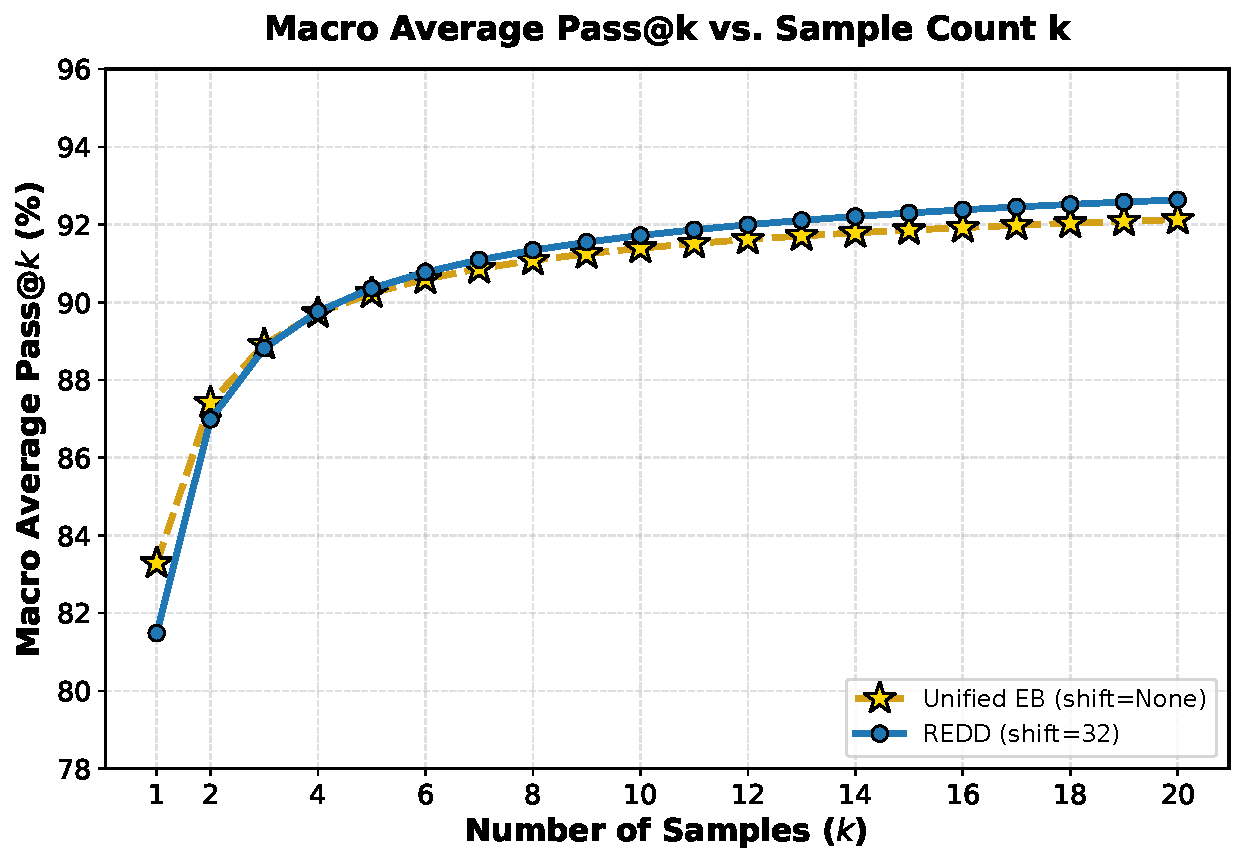
\includegraphics[width=\linewidth]{images/fig_macro_pass_at_k.pdf}
\captionof{figure}{\textbf{Macro Average Pass@$k$ vs.\ Sample Count $k$}. While Unified EB achieves higher Pass@1, RES ($s=32$; ``Rolling'' in the legend) exhibits stronger multi-sample scaling, overtaking Unified EB at $k \ge 6$ to reach $93.58\%$ Pass@20 while running $+31.3\%$ faster.}
\label{fig:macro_pass_at_k}

\end{minipage}
\par\vspace{12pt}
\begin{minipage}{\textwidth}
\centering
    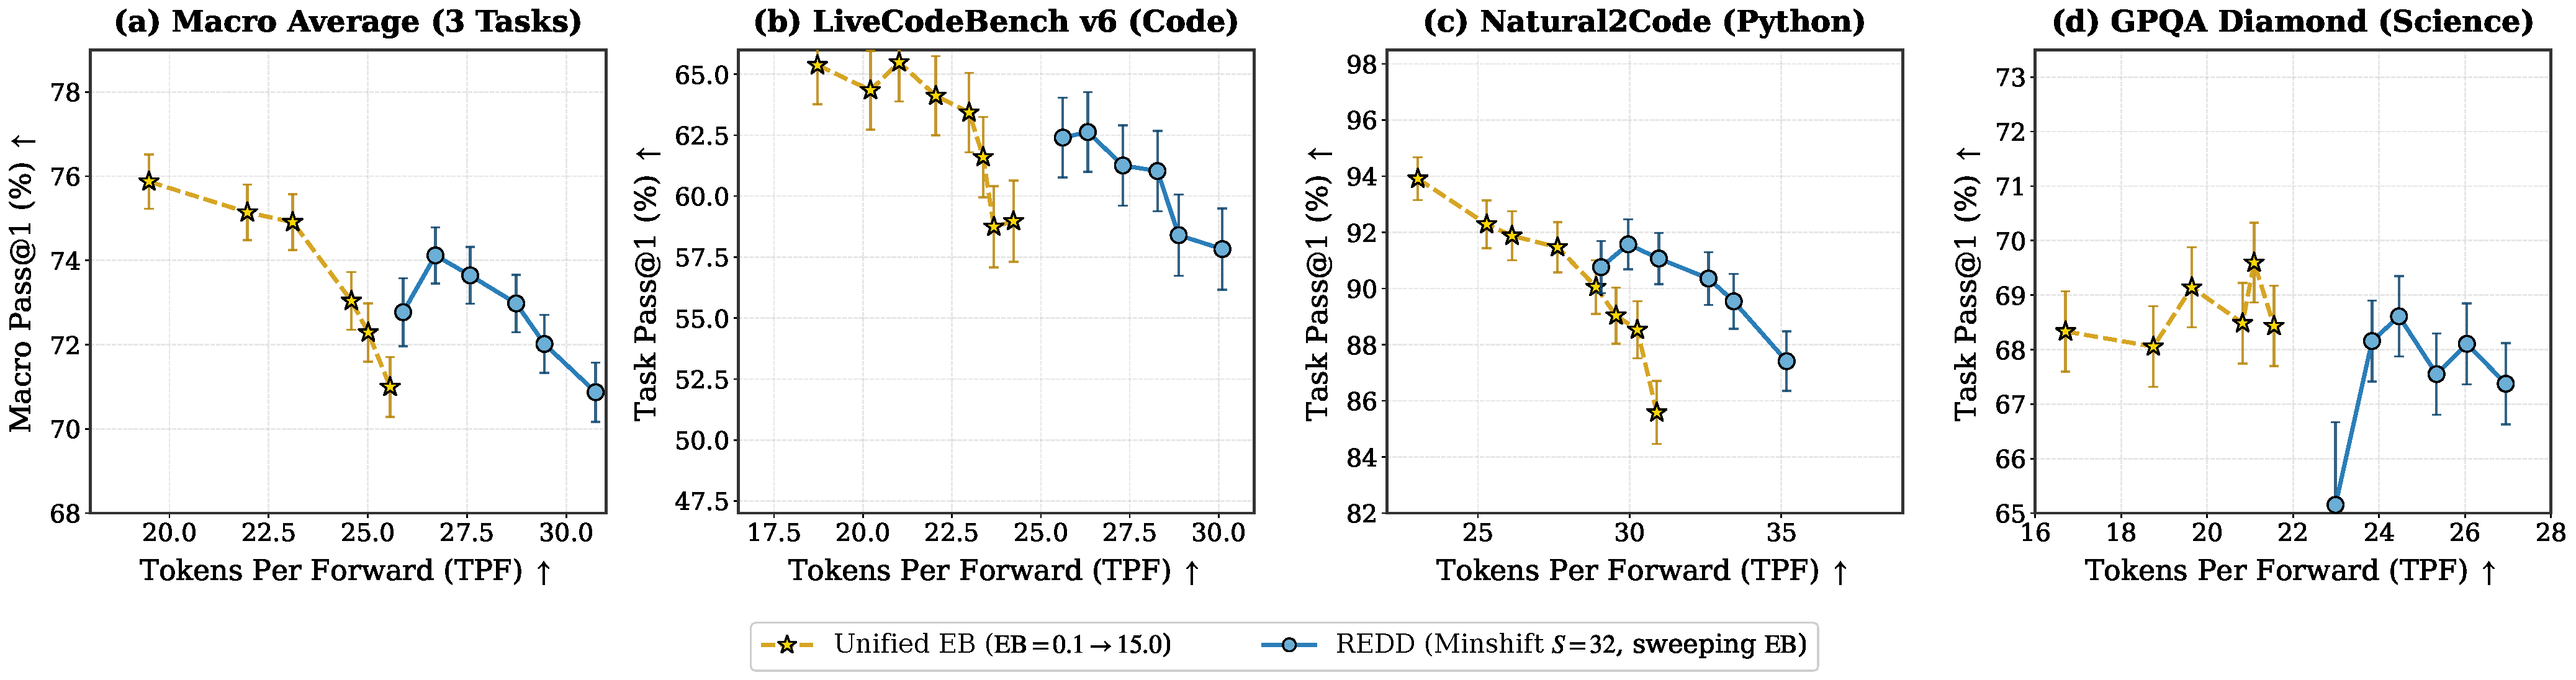
\includegraphics[width=\linewidth]{images/fig_merged_minshift32_eb01_1x4_row.pdf}
    \captionof{figure}{Pareto frontiers of RES with minimum shift $s=32$ (``Merged Sampler'') and Unified EB (``Standard EB Baseline'') under varied EB bounds $.05 \to 1.0$ for LCB v6 and Natural2Code with 5 seed averages, and GPQA Diamond with 20 seed averages due to high noise in the eval.}
    \label{fig:minshift-16}

\end{minipage}
\end{minipage}
\end{lrbox}
